\documentclass[11pt,a4paper]{article}
\usepackage[utf8]{inputenc}
\usepackage{amsmath,amssymb,amsthm}
\usepackage{geometry}
\usepackage{booktabs}
\usepackage{tabularx}
\usepackage{hyperref}
\usepackage{microtype}
\usepackage{tikz}
\usepackage{pgfplots}
\pgfplotsset{compat=1.18}
\usetikzlibrary{arrows,positioning,shapes.geometric,calc}

\geometry{margin=1in}

\hypersetup{
    colorlinks=true,
    linkcolor=blue,
    citecolor=blue,
    urlcolor=blue,
    pdftitle={Deep Dive: Theorem A' --- Source-Channel Latent-Class Identifiability},
    pdfauthor={Arben Lila}
}

\usepackage[firstpage=false]{draftwatermark}
\DraftwatermarkOptions{text={SUPERSEDED DRAFT\\DO NOT CITE},color=red!25,angle=55,scale=1.2}

\newtheorem{theorem}{Theorem}
\newtheorem{lemma}[theorem]{Lemma}
\newtheorem{definition}{Definition}
\newtheorem{claim}[theorem]{Claim}

\title{\textbf{A Pedagogical Deep Dive into Theorem $A'$}\\
\large Source-Channel Latent-Class Identifiability in the DAVID/M0.1 Engine}
\author{\textbf{Arben Lila} \\ \textit{Internal Thesis Work}}
\date{\today}

\begin{document}

\maketitle

\begin{abstract}
This report provides a comprehensive, self-contained mathematical and conceptual exposition of Theorem $A'$ (Source-Channel Latent-Class Identifiability), the foundational gatekeeper of the DAVID/M0.1 predictive engine. We resolve the circularity paradox of latent state estimation and source reliability calibration, detail each model parameter, and present the step-by-step mathematical proof based on Kruskal's tensor decomposition uniqueness theorem (1977). Furthermore, we analyze the degrees of freedom constraint comparing $S=2$ and $S=3$ observers, and demonstrate how the engine's operational diagnostics guard against real-world failures such as conditional source dependence, information collapse, and label switching.
\end{abstract}

\tableofcontents
\newpage

\section{The Circularity Paradox (Intuition)}
When modeling hidden events in policy monitoring (such as Tobacco Industry interference or policy obstruction), we are confronted with a fundamental challenge: the true state of interest is a \textbf{latent variable}. It exists in reality but cannot be measured directly with $100\%$ certainty. We denote this state as $A \in \{0, 1\}$.

To monitor this latent state, we deploy $S$ noisy, imperfect sources (e.g., local RSS scrapers, legislative databases, and LLM classifiers). Each source $s$ has unknown performance characteristics:
\begin{itemize}
    \item A true positive rate (sensitivity) $\rho_s$, representing how likely it is to flag active obstruction.
    \item A false positive rate $\delta_s$, representing how likely it is to raise a false alarm.
\end{itemize}

This leads to a \textbf{circularity paradox} (the ``chicken-and-egg'' problem):
\begin{enumerate}
    \item To know how reliable a source is ($\rho_s, \delta_s$), we must know the true state of the world ($A$).
    \item To know the true state of the world ($A$), we must know the reliability of our sources ($\rho_s, \delta_s$).
\end{enumerate}

If we do not know either, is it possible to unique recover both parameters simultaneously? Or are there infinite different combinations of source reliability profiles and true prevalence states that generate the exact same observed data?

Theorem $A'$ resolves this paradox. It mathematically guarantees that as long as we observe at least **three conditionally independent sources**, the parameters are uniquely identifiable up to a simple swap of the state labels.

---

\section{Parameter Glossary}
To anchor the mathematical proofs, we define each parameter and its corresponding domain in Table~\ref{tab:parameters}.

\begin{table}[h]
\centering
\caption{Model parameters and their operational definitions under the Kosovo Smoke-Free policy stratum.}
\label{tab:parameters}
\begin{tabularx}{\textwidth}{llX}
\toprule
\textbf{Parameter} & \textbf{Mathematical Definition} & \textbf{Kosovo Case Study Meaning} \\
\midrule
$A \in \{0, 1\}$ & Latent binary activity state & Is TI actively obstructing the policy? (1 = Yes, 0 = No) \\
$\phi \in [0, 1]$ & State prevalence prior: $P(A = 1)$ & True underlying probability of obstruction. \\
$Y_s \in \{0, 1\}$ & Observed binary label from source $s$ & Did Source $s$ (e.g., RSS, LLM) report obstruction? \\
$\rho_s \in [0, 1]$ & Sensitivity: $P(Y_s = 1 \mid A = 1)$ & True Positive Rate of source $s$. \\
$\delta_s \in [0, 1]$ & False positive rate: $P(Y_s = 1 \mid A = 0)$ & Noise rate of source $s$. \\
$T_{ijk} \in [0, 1]$ & Joint probability $P(Y_1=i, Y_2=j, Y_3=k)$ & Observed frequency of joint source configurations. \\
\bottomrule
\end{tabularx}
\end{table}

---

\section{Step-by-Step Mathematical Proof}
We observe only the joint outputs of our sources. For $S=3$ binary sources, we can measure how often we see the 8 possible joint outcomes: $(0,0,0), (1,0,0), \dots, (1,1,1)$. This joint distribution forms a $2 \times 2 \times 2$ grid of numbers, which is a \textbf{three-way tensor} denoted by $T \in \mathbb{R}^{2 \times 2 \times 2}$, where $T_{ijk} = P(Y_1=i, Y_2=j, Y_3=k)$.

\subsection{Step 1: Writing the Tensor CP Decomposition}
By the assumption of \textbf{conditional independence}, the sources do not communicate; their outputs are independent once conditioned on the latent state $A$. Thus, for any cell $(i, j, k) \in \{0, 1\}^3$:
\begin{equation}\label{eq:joint_prob}
T_{ijk} = \sum_{a \in \{0, 1\}} P(A = a) P(Y_1=i \mid A=a) P(Y_2=j \mid A=a) P(Y_3=k \mid A=a)
\end{equation}

For each source $s$, we define a conditional probability matrix $M^{(s)} \in \mathbb{R}^{2 \times 2}$ where the columns represent the class-conditional distributions:
\[
M^{(s)} = \begin{pmatrix} 
P(Y_s=0 \mid A=0) & P(Y_s=0 \mid A=1) \\ 
P(Y_s=1 \mid A=0) & P(Y_s=1 \mid A=1) 
\end{pmatrix} = \begin{pmatrix} 
1 - \delta_s & 1 - \rho_s \\ 
\delta_s & \rho_s 
\end{pmatrix}
\]
Let $\boldsymbol{\pi} = \begin{pmatrix} 1 - \phi \\ \phi \end{pmatrix}$ be the latent state distribution vector. We can rewrite Equation~\eqref{eq:joint_prob} in tensor notation:
\[
T_{ijk} = \sum_{a=0}^{1} \pi_a M^{(1)}_{ia} M^{(2)}_{ja} M^{(3)}_{ka}
\]
This is a **Canonical Polyadic (CP) tensor decomposition** of the observed joint distribution $T$ into a sum of $R=2$ rank-1 tensors.

\subsection{Step 2: Kruskal Rank of the Source Channels}
Kruskal (1977) proved that the CP decomposition of a 3-way tensor is unique under mild algebraic conditions. We define the **Kruskal rank** (or $k$-rank) of a matrix:
\begin{definition}
The Kruskal rank $k(M)$ of a matrix $M$ is the largest integer $k$ such that any $k$ columns of $M$ are linearly independent.
\end{definition}

For our $2 \times 2$ factor matrices $M^{(s)}$, the columns are linearly independent (implying $k(M^{(s)}) = 2$) if and only if the matrix has full rank. This holds if and only if the determinant is non-zero:
\[
\det(M^{(s)}) = (1 - \delta_s)\rho_s - (1 - \rho_s)\delta_s = \rho_s - \delta_s
\]
Thus, the Kruskal rank is $2$ if and only if:
\[
\rho_s \neq \delta_s
\]
This condition means the source channel is non-degenerate (i.e., the source is not a random coin flip). If this holds for all three sources:
\[
k(M^{(1)}) = k(M^{(2)}) = k(M^{(3)}) = 2
\]

\subsection{Step 3: Evaluating Kruskal's Uniqueness Bound}
Kruskal's theorem states that the CP decomposition of a 3-way tensor with $R$ components is unique up to permutation and scaling of the factor columns if:
\begin{equation}\label{eq:kruskal_theorem_bound}
k(M^{(1)}) + k(M^{(2)}) + k(M^{(3)}) \ge 2R + 2
\end{equation}

For $R = 2$ latent classes, the right-hand side of Equation~\eqref{eq:kruskal_theorem_bound} is:
\[
2R + 2 = 2(2) + 2 = 6
\]
Summing our actual Kruskal ranks:
\[
k(M^{(1)}) + k(M^{(2)}) + k(M^{(3)}) = 2 + 2 + 2 = 6
\]
Since $6 \ge 6$, the uniqueness bound is satisfied. Consequently, the parameters $(\phi, \{\rho_s, \delta_s\}_{s=1}^3)$ are uniquely identifiable from the joint distribution $T$ up to a simple swap of the latent labels $0$ and $1$. \qed

---

\section{Degrees of Freedom Analysis: $S=2$ vs $S=3$}
We can understand this intuitively by comparing the number of independent equations (observations) to the number of unknowns (parameters).

\subsection{The Case of $S=2$ Sources (Unidentifiable)}
With two binary sources $Y_1, Y_2$, the joint probability table contains $2^2 = 4$ cells. Since the probabilities must sum to 1, we have $4 - 1 = \mathbf{3}$ independent equations.
We are trying to estimate:
* The prior: $\phi$ (1 parameter)
* Channel 1: $\rho_1, \dots$ (2 parameters)
* Channel 2: $\rho_2, \dots$ (2 parameters)
* **Total unknowns = 5**

A system with 3 equations and 5 unknowns has infinitely many solutions. We cannot identify the true parameters.

\subsection{The Case of $S=3$ Sources (Identifiable)}
With three binary sources, the joint table has $2^3 = 8$ cells, providing $8 - 1 = \mathbf{7}$ independent equations.
We are trying to estimate:
* The prior: $\phi$ (1 parameter)
* Channel 1: $\rho_1, \delta_1$ (2 parameters)
* Channel 2: $\rho_2, \delta_2$ (2 parameters)
* Channel 3: $\rho_3, \delta_3$ (2 parameters)
* **Total unknowns = 7**

We have 7 equations and 7 unknowns. The system is fully determined, allowing a unique mathematical solution.

---

\section{Resilience to Challenges}

\subsection{Challenge 1: Conditional Source Dependence (Collusion)}
If sources share information (e.g., Source 2 copy-pastes Source 1's reports), the conditional independence assumption fails:
\[
P(Y_1, Y_2 \mid A) \neq P(Y_1 \mid A)P(Y_2 \mid A)
\]
In this case, the tensor structure is corrupted. The model will overestimate the information content, narrowing the posterior unnaturally and biasing the activity estimates.

\begin{figure}[h]
\centering
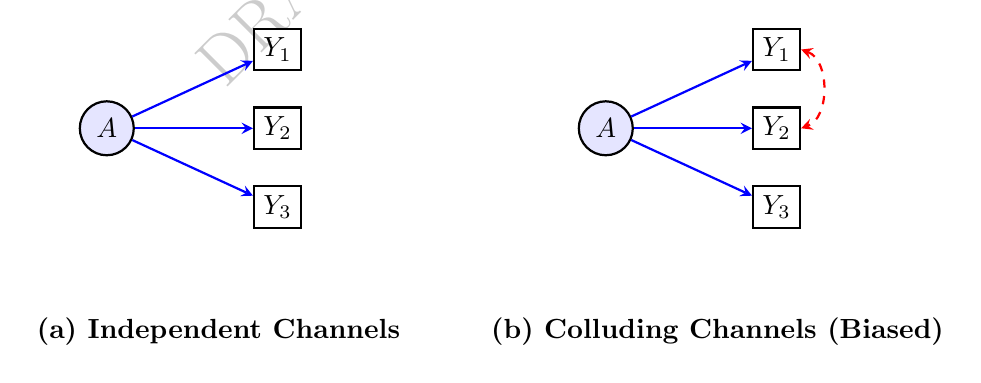
\begin{tikzpicture}[node distance=1.5cm, >=stealth, thick]
    % Left side: Independent
    \node[circle, draw, fill=blue!10] (A1) {$A$};
    \node[rectangle, draw, right=of A1, yshift=1cm] (Y11) {$Y_1$};
    \node[rectangle, draw, right=of A1] (Y12) {$Y_2$};
    \node[rectangle, draw, right=of A1, yshift=-1cm] (Y13) {$Y_3$};
    \draw[->, blue] (A1) -- (Y11);
    \draw[->, blue] (A1) -- (Y12);
    \draw[->, blue] (A1) -- (Y13);
    \node[below=1.0cm of Y13, xshift=-0.75cm] {\textbf{(a) Independent Channels}};

    % Right side: Dependent
    \node[circle, draw, fill=blue!10, right=of Y12, xshift=2cm] (A2) {$A$};
    \node[rectangle, draw, right=of A2, yshift=1cm] (Y21) {$Y_1$};
    \node[rectangle, draw, right=of A2] (Y22) {$Y_2$};
    \node[rectangle, draw, right=of A2, yshift=-1cm] (Y23) {$Y_3$};
    \draw[->, blue] (A2) -- (Y21);
    \draw[->, blue] (A2) -- (Y22);
    \draw[->, blue] (A2) -- (Y23);
    \draw[<->, red, dashed] (Y21.east) to [bend left=70] (Y22.east);
    \node[below=1.0cm of Y23, xshift=-0.75cm] {\textbf{(b) Colluding Channels (Biased)}};
\end{tikzpicture}
\caption{Graphical models of source channels. The red dashed line represents conditional dependence (collusion), which breaks the tensor CP decomposition structure.}
\label{fig:channels}
\end{figure}

* **Engine Defense:** The engine audits the sources using the Source Independence Ledger (\texttt{config/source\_independence.json}). If two sources are structurally linked, their joint likelihood is penalized or merged to prevent bias.

\subsection{Challenge 2: Channel Degeneracy (Noise)}
If a source $s$ degenerates into random noise, its sensitivity and false positive rate converge: $\rho_s \to \delta_s$. As a result:
\[
\det(M^{(s)}) \to 0 \implies k(M^{(s)}) \to 1
\]
The sum of Kruskal ranks collapses to $2 + 2 + 1 = 5$, violating the uniqueness bound ($5 < 6$). Identifiability is lost, and the MCMC sampler will fail to converge, exhibiting wide, uninformative posteriors.

* **Engine Defense:** The engine computes the **Practical Identification Distance** $d(\theta)$ at every iteration. If the distance drops below $0.05$, Gate **FG2** fail-closes, blocking the stratum and routing it to \texttt{evidence\_gap}.

\begin{figure}[h]
\centering
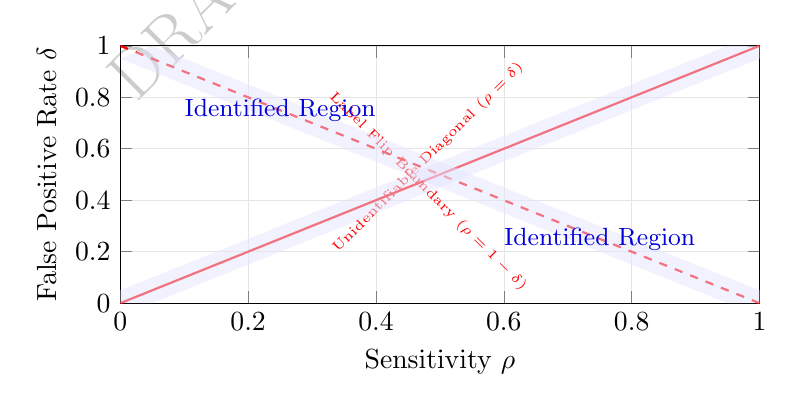
\begin{tikzpicture}
\begin{axis}[
    width=0.8\textwidth,
    height=0.4\textwidth,
    xlabel={Sensitivity $\rho$},
    ylabel={False Positive Rate $\delta$},
    xmin=0, xmax=1,
    ymin=0, ymax=1,
    grid=both,
    grid style={line width=.1pt, draw=gray!10},
    major grid style={line width=.2pt, draw=gray!20},
]
% Diagonal line (completely unidentifiable)
\addplot[thick, red, domain=0:1] {x};
\node[anchor=south, rotate=45, text=red, font=\tiny] at (axis cs: 0.5, 0.52) {Unidentifiable Diagonal ($\rho = \delta$)};

% Anti-diagonal line
\addplot[thick, red, dashed, domain=0:1] {1-x};
\node[anchor=north, rotate=-45, text=red, font=\tiny] at (axis cs: 0.5, 0.48) {Label Flip Boundary ($\rho = 1-\delta$)};

% Highlight region of practical identifiability (d >= 0.05)
\fill[blue!10, opacity=0.5] (axis cs: 0, 0.05) -- (axis cs: 0.95, 1) -- (axis cs: 1, 1) -- (axis cs: 1, 0.95) -- (axis cs: 0.05, 0) -- (axis cs: 0, 0) -- cycle;
\fill[blue!10, opacity=0.5] (axis cs: 0, 0.95) -- (axis cs: 0.05, 1) -- (axis cs: 1, 0.05) -- (axis cs: 1, 0) -- (axis cs: 0.95, 0) -- cycle;

\node[text=blue!85!black, font=\small] at (axis cs: 0.25, 0.75) {Identified Region};
\node[text=blue!85!black, font=\small] at (axis cs: 0.75, 0.25) {Identified Region};

\end{axis}
\end{tikzpicture}
\caption{Parameter space of source channels. The solid red line represents complete degeneracy. The blue shaded regions represent the mathematically identified spaces enforced by Gate FG2 ($d(\theta) \ge 0.05$).}
\label{fig:parameter_space}
\end{figure}

\end{document}
